\documentclass[a4paper]{article}

\usepackage{parskip}
\usepackage{setspace}
\usepackage{fullpage}
\usepackage{graphicx}

\begin{document}

\title{Planning, Estimating and Tracking}
\author{Andrew Higginson \and Bryan Liu \and Choo Jia Guang \and Emma Hulme \and Timothy 'The Power' van Bremen \and Thomas Taylor-Hall}
\date{October 2014}
\maketitle

\linespread{1.1}

\section{Project Introduction}
As part of the renovation of the William Penney Building on the Sherfield 
walkway, interactive screens are to be installed. Mounted inside the building, 4
projectors will simulataneously display content onto floor to ceiling glass
panels that are visible to passers-by. Also, an 84-inch 4K resolution touch 
screen is to be mounted by the entrance doors. 

Our project consists of developing an "App Store" for uploading images and 
interactive content to be displayed on the 4 projected screens. Also, we will be
developing a playout system to show the content on multiple screens in multiple 
resolutions.

\section{User Requirements} \label{section:req}

SEE GOOGLE DOC FOR THIS!


\section{Project Plan}
Current plan and how we can adapt it:
	- agreed on estimation of amount of time it takes to ocmplete tasls
  - timeline
  - leeway for problems (experience from previous projects)

How did we come up with it? 
	- identifying components
	- taking into account other 

\subsection{Task Estimation}
The group is acutely aware that with Computing examinations being held at the
end of term, we could only practically carry out development work until the
first week of December. Furthermore, committments in other courses mean that 
each team member is only able to devote around 16-20 hours per week to
the project.

Based on such constraints, we have decided to commit to the following:
\begin{enumerate}
  \item To maintain a 1-week iteration: this allows the development team to
        obtain maximum possible feedback from the client/supervisor.
  \item To strictly adhere to original project scope: while we believe the
        current scope is managable, we would reject time-consuming items which
        are out of scope unless a minimal working system is implemented.
\end{enumerate}


\begin{figure}[h]
  \centering
    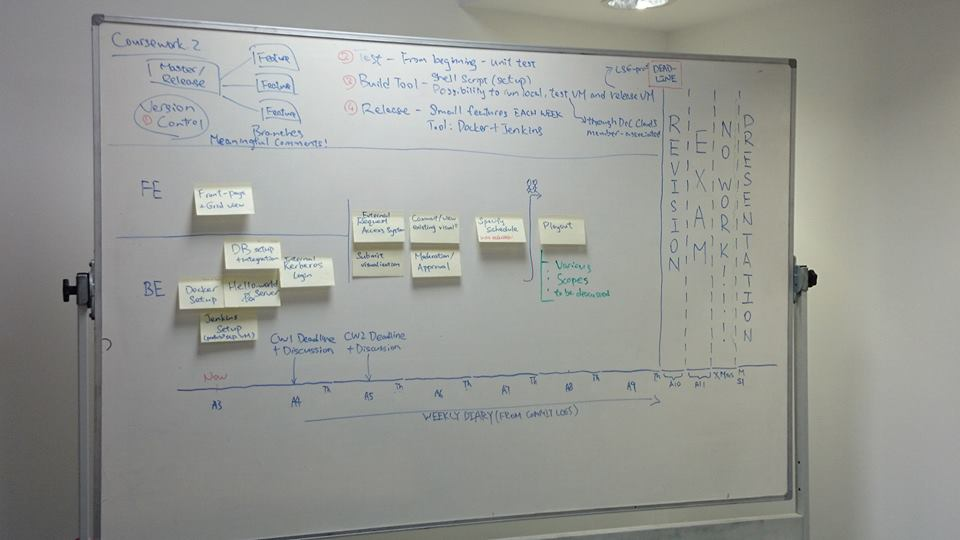
\includegraphics[width = 0.99\textwidth]{./planning/timeline.jpg}
   
  \caption{Project plan with timeline.}
  \label{fig:timeline}
\end{figure}

% Estimation & Planning - Iteration Plans + Release Plans
The resultant plan and timeline shown in figure \ref{fig:timeline} is a
combination of the plan for next iteration and the release plan, taking account
of the current project scope. Each post-it note either represents a 
concrete task to be completed during the next iteration (towards the left), or
high level themes to be implemented (towards the right). Each line segment at
the bottom represents an iteration ending on Thursday, when the development
team will meet with the client.

% Estimation & Planning - T-Shirt Sizing
Estimates on time required for the tasks were based on their relative size and
time taken for us to complete similar ones in the past. For example, some of us
have implemented a College (Kerberos) Login System well within a week, thus if
it is a size M, we can infer that the team (now double the size) is capable in 
fitting two size M tasks within an iteration. For larger system modules, we
assign a longer period specifically for that task: we expect the scheduling
system (size L) and the entire playout system (size XL) would take us one and
two iteration(s) respectively.


\subsection{Group organisation}
After we established the requirements of the project, each group member stated
which part of the project they would like to work on. We found that there was a
good split of two people that wanted to work on the frontend, two on the backend
server code, and two on the database.

Although this is a good split to initiate work, we realised that the frontend 
aspect of the project may require more work in the long term. In addition, we 
expect that the server code and database should be fully implemented a few
weeks before the frontend is completed, only requiring minor fixes.

Therefore, we decided that two people from the backend would move on to creating
the playout software on the dedicated computers; one person would help with the
frontend and the remaining person would apply small fixes and refactors to the
existing server/database code. 


\subsection{Development Methods \& Project Tracking}
  - using trello (physical story board not feasible, kanban)
  - constantly communicating (messaging software, regular stand-ups)

\subsection{Development Tools}
 	- Flask for the backend as it's new and interesting, lightweight
	- bryan wanted to experiment with MongoDB
	- AngularJS for frontend for interest's sake
	- Docker as we want to deploy on multiple virtual machines using cloudstack
	- can test backend if frontend has changed and is not working
  - David's VM
	- dedicated comps to run playout software



\end{document}
